\chapter{Hipercuádricas afines}

\begin{definicion}
    Sea $\cc{A}^n$ un espacio afín, y $\cc{R}$ un sistema de referencia. Definimos una hipercuádrica afín real $H$ como:
    \begin{equation*}
        H = \left\{p\in \cc{A} ~:~ (1,p_{\cc{R}}^t) \cdot \wh{C} \cdot \left(\begin{array}{c}
            1 \\ p_{\cc{R}}
        \end{array}\right) = 0\right\}
    \end{equation*}
    donde $\wh{C}=\left(\begin{array}{c|c}
        a & z^t \\ \hline
        z & C
    \end{array}\right)\in \cc{S}_{n+1}(\bb{R})$, donde $a\in \bb{R}$, $z\in \bb{R}^n$ y $C\in \cc{S}_{n}(\bb{R})\setminus \{0\}$.

    A la matriz $\wh{C}$ la llamaremos la matriz asociada a $H$ en $\cc{R}$.
\end{definicion}

Sea ahora $p_\cc{R} = (x_1,\dots,x_n)^t$, $z=(z_1,\dots,z_n)^t$ y $C=(c_{ij})_{i,j=1,\dots,n}$, con $c_{ij} = c_{ji}$ por ser $C\in \cc{S}_{n}(\bb{R})\setminus \{0\}$. Veamos en primer lugar que $H$ está muy relacionado con las formas cuadráticas vistas en Geometría II:
\begin{equation*}\begin{split}
    0=(1, p_{\cc{R}}^t)\left(\begin{array}{c|c}
        a & z^t \\ \hline
        z & C
    \end{array}\right)&\left(\begin{array}{c}
        1 \\ p_{\cc{R}}
    \end{array}\right) = 
    (a + p_{\cc{R}}^tz, z^t + p_{\cc{R}}^tC)\left(\begin{array}{c}
        1 \\ p_{\cc{R}}
    \end{array}\right)
    =\\&= a + p_{\cc{R}}^tz + z^tp_{\cc{R}} + p_{\cc{R}}^tCp_{\cc{R}}
    = a + 2p_{\cc{R}}^tz + p_{\cc{R}}^tCp_{\cc{R}}
\end{split}\end{equation*}
donde tenemos que $p_{\cc{R}}^tCp_{\cc{R}}$ era la forma cuadrática asociada a la métrica definida por la matriz $C$ en la base $\cc{B}$.

Análogamente, tenemos que $H$ se corresponde con una ecuación cuadrática\footnote{Recordemos que una ecuación cuadrática es, simplemente, un polinomio de grado 2.}, que resulta menos abstracto:
\begin{equation*}\begin{split}
    0 =&~a + 2p_{\cc{R}}^tz + p_{\cc{R}}^tCp_{\cc{R}} =\\&=a + 2(x_1,\dots,x_n)\left(\begin{array}{c}
        z_1 \\ \vdots \\ z_n
    \end{array}\right)
    + (x_1,\dots,x_n)
    \left(\begin{array}{ccc}
        c_{11} & \cdots & c_{1n} \\
        \vdots& \ddots & \vdots \\
        c_{1n}& \cdots & c_{nn}
    \end{array}\right)
    \left(\begin{array}{c}
        x_1 \\ \vdots \\ x_n
    \end{array}\right)
    =\\&= a + 2\sum_{i=1}^nz_ix_i + \sum_{i,j=1}^n c_{ij}x_ix_j 
\end{split}\end{equation*}

\begin{ejemplo}
    Sea $\cc{A}^n$ un espacio afín, y $\cc{R}$ un sistema de referencia. Encontrar la ecuación cuadrática de la hipercuádrica $H$, cuya matriz asociada en $\cc{R}$ es la siguiente:
    \begin{equation*}
        A = \left(\begin{array}{c|cc}
            1 & 1 & 2 \\ \hline
            1 & 0 & 1 \\
            2 & 1 & 1
        \end{array}\right)
    \end{equation*}

    Tenemos que $H=\{(x,y)_\cc{R}\in \cc{A} \mid y^2 + 2xy + 2x+4y+1=0\}$.
\end{ejemplo}

\section{Cambio de sistema de referencia e hipercuádricas}

Como hemos visto, las hipercuádricas se han definido según un sistema de referencia $\cc{R}$; por lo que es lógico preguntarse cómo se ven modificados si dicho sistema de referencia cambia.

Además del sistema de referencia $\cc{R}=\{p_0,\cc{B}\}$ que se ha considerado para definir una hipercuádrica, sea $\cc{R}'=\{p_0', \cc{B}'\}$ otro sistema de referencia tal que:
\begin{equation*}
    M(Id_{\cc{A}}, \cc{R}', \cc{R}) = \left(\begin{array}{c|c}
        1 & 0 \\ \hline
        b & A
    \end{array}\right),\hspace{1cm} A = M(\cc{B}', \cc{B})
\end{equation*}

Entonces, tenemos que:
\begin{equation*}\begin{split}
    0=&(1, p_{\cc{R}}^t)\left(\begin{array}{c|c}
        a & z^t \\ \hline
        z & C
    \end{array}\right)\left(\begin{array}{c}
        1 \\ p_{\cc{R}}
    \end{array}\right)
    =\\=& (1, p_{\cc{R}'}^t)\left(\begin{array}{c|c}
        1 & b^t \\ \hline
        0 & A^t
    \end{array}\right)\left(\begin{array}{c|c}
        a & z^t \\ \hline
        z & C
    \end{array}\right)\left(\begin{array}{c|c}
        1 & 0 \\ \hline
        b & A
    \end{array}\right)\left(\begin{array}{c}
        1 \\ p_{\cc{R}'}
    \end{array}\right) =\\
    =& (1, p_{\cc{R}'}^t)\left(\begin{array}{c|c}
        a+b^tz & z^t+b^tC \\ \hline
        A^tz & A^tC
    \end{array}\right)\left(\begin{array}{c|c}
        1 & 0 \\ \hline
        b & A
    \end{array}\right)\left(\begin{array}{c}
        1 \\ p_{\cc{R}'}
    \end{array}\right)
    =\\
    =& (1, p_{\cc{R}'}^t)\left(\begin{array}{c|c}
        a+b^tz + z^tb+b^tCb & z^tA + b^tCA\\ \hline
        A^tz+A^tCb & A^tCA
    \end{array}\right)\left(\begin{array}{c}
        1 \\ p_{\cc{R}'}
    \end{array}\right)=\\
    =& (1, p_{\cc{R}'}^t)\left(\begin{array}{c|c}
        \wt{a} & \wt{z}^t\\ \hline
        \wt{z} & A^tCA
    \end{array}\right)\left(\begin{array}{c}
        1 \\ p_{\cc{R}'}
    \end{array}\right)
\end{split}\end{equation*}

Por tanto, se tiene que:
\begin{equation*}
    \left\{\begin{array}{l}
        \wt{a} = a+b^tz + z^tb + b^tCb \\
        \wt{z} = A^t(Cb+z)
    \end{array}\right.
\end{equation*}


\section{Clasificación de hipercuádricas euclídeas}

Dada una hipercuádrica euclídea, nuestro objetivo es encontrar un sistema de referencia en el que la ecuación cuadrática sea fácil de identificar, pudiendo entonces clasificarla.

\begin{definicion}
    Sean $C_1$, $C_2$ dos hipercuádricas de $\bb{R}^n$. Decimos que $C_1$ y $C_2$ son \emph{equivalentes} si existe una biyección $f:\bb{R}^n\to \bb{R}^n$ tal que $f(C_1)=C_2$.
\end{definicion}

La siguiente proposición es de demostración sencilla, ya que la composición de biyecciones es una biyección, y la inversa de una biyección es una biyección.
\begin{prop}
    Sea $\cc{A}$ un espacio afín. En el conjunto de todas las hipercuádricas de $\cc{A}$, la relación ``ser equivalente a'' es una relación de equivalencia.
\end{prop}

En esta sección nos vamos a centrar en clasificar las hipercuádricas euclídeas mediante cambios de sistema de referencia, que son biyecciones.

Por el Teorema de Sylvester visto en Geometría II, como $C$ es simétrica, tenemos que $\exists \cc{B}'$ base ortonormal de $\vec{\cc{A}}$ tal que $A^tCA=D$, con $D$ diagonal:
\begin{equation*}
    D=A^tCA = \left(
    \begin{array}{ccc|ccc|ccc}
       r_1&&&&&&&& \\
       & \ddots&&&&&&&\\
       && r_{n_1}&&&&&&\\ \hline
       &&& -r_{n_1+1}&&&&&\\
       &&&& \ddots&&&&\\
       &&&&& -r_{n_1+n_2}&&&\\ \hline
       &&&&&& 0&&\\
       &&&&&&& \ddots &\\
       &&&&&&&& 0
    \end{array}
    \right)
\end{equation*}
donde $r_k>0$ para todo $k=1,\dots,n_1+n_2$. Además, veamos que se puede elegir $b$ de la forma que $\wt{z}$ (que también define la hipercuádrica) tenga sus primeras $n_1+n_2$ coordenadas nulas.
\begin{comment}
Tenemos que $A^tz$ es un vector columna, por lo que sea $A^tz=\lm$:
\begin{equation*}
    \left(\begin{array}{c}
        0 \\ \vdots \\ 0 \\ z_{n_1+n_2+1} \\ \vdots \\ z_n
    \end{array}\right) = \wt{z}= A^tz+A^tCb = \lm+DA^tb = \left(\begin{array}{c}
        \lm_1 \\ \vdots \\ \lm_{n_1+n_2} \\ \lm_{n_1+n_2+1} \\ \vdots \\ \lm_n
    \end{array}\right)+DA^tb
\end{equation*}
\end{comment}


Por tanto, hay un sistema de referencia ortonormal $\cc{R}'$ tal que $H$ viene dada por:
\begin{equation*}
    0 = (1, p_{\cc{R}'}^t)\left(
    \begin{array}{c|ccc|ccc|ccc}
        \wt{a} &&0&&&0&&\wt{z}_{n_1+n_2+1}&\cdots&\wt{z}_{n}   \\ \hline
        &r_1&&&&&&&& \\
        0&& \ddots&&&&&&&\\
        &&& r_{n_1}&&&&&&\\ \hline
        &&&& -r_{n_1+1}&&&&&\\
        0&&&&& \ddots&&&&\\
        &&&&&& -r_{n_1+n_2}&&&\\ \hline
        \wt{z}_{n_1+n_2+1}&&&&&&& 0&&\\
        \vdots&&&&&&&& \ddots &\\
        \wt{z}_n&&&&&&&&& 0
    \end{array}
    \right)\left(\begin{array}{c}
        1 \\ p_{\cc{R}'}
    \end{array}\right)
\end{equation*}
donde $r_k>0$ para todo $k=1,\dots,n_1+n_2$. Distinguimos ahora en función de si $\wt{z}$ es nulo o no:
\begin{enumerate}
    \item \ul{El vector columna $\wt{z}$ es nulo, $\wt{z}=\vec{0}$}:

    En este caso, si $p_{\cc{R}'}^t = (s_1,\dots,s_n)$, los puntos de $H$ cumplen:
    \begin{equation*}
        r_1s_1^2 + \dots + r_{n_1}s_{n_1}^2 - r_{n_1+1}s_{n_1+1}^2 - r_{n_1+n_2}s_{n_1+n_2}^2 = -\wt{a}
    \end{equation*}
    donde $r_k>0$ para todo $k=1,\dots,n_1+n_2$. Además, podemos suponer que el número de coeficientes positivos es mayor o igual que el número de valores negativos, cambiando de signo la igualdad si hiciese falta. Además, si $\wt{a}\neq 0$, podemos dividir entre $\wt{a}$ de forma que esté igualado a $\pm 1$. Por tanto, haciendo esos cambios tenemos que:
    \begin{equation*}
        R_1s_1^2 + \dots + R_{m}s_{m}^2 - R_{m+1}s_{m+1}^2 - R_{l}s_{l}^2 = \veps
    \end{equation*}
    donde los $R_i$ son números positivos, $m \geq \nicefrac{l}{2}$ y $\veps\in\{-1, 0, 1\}$.

    Por último, veamos que si $\veps=0$, podemos dividir entre $R_l$ de manera que el coeficiente de $s_l^2$ sea $1$.

    \item \ul{El vector columna $\wt{z}$ no es nulo, $\wt{z}\neq \vec{0}$}:

    Ya que $\wt{w}^t = (\wt{z}_{n_1+n_2+1},\dots, \wt{z}_{n})_{\cc{B}'}\neq \vec{0}$, ampliamos a una base ortonormal de $\bb{R}^{n-(n_1+n_2)}$ dada por $\cc{B}''_{\wt{w}}=\{e_{n_1+n_2+1}, \dots, e_n\}$, con $e_n = \frac{\wt{w}}{\|\wt{w}\|}$. Por tanto, consideramos el sistema de referencia $\cc{R}''$ tal que:
    \begin{equation*}
        M(Id_{\cc{A}}, \cc{R}'', \cc{R}') = \left(\begin{array}{c|c|c}
            1 & 0 & 0 \\ \hline
            0 & I_{n_1+n_2} & 0 \\
            0 & 0 & B
        \end{array}\right)
    \end{equation*}
    donde $B=M(\cc{B}''_{\wt{w}}, \cc{B}'_{\wt{w}})$ y $\cc{B}'_{\wt{w}}$ son los $n-(n_1+n_2)$ últimos vectores de $\cc{B}'$.

    Como en este caso $\wt{b}=0$, tenemos que $\wt{\wt{z}} = B^t\wt{w} = (0,\dots, 0, \|w\|)^t$. Por tanto, en $\cc{R}''$ tenemos que $H$ viene dada por:
    \begin{equation*}
        0 = (1, p_{\cc{R}''}^t)\left(
        \begin{array}{c|ccc|ccc|ccc}
            \wt{\wt{a}} &&0&&&0&&0&\cdots&\|w\|   \\ \hline
            &r_1&&&&&&&& \\
            0&& \ddots&&&&&&&\\
            &&& r_{n_1}&&&&&&\\ \hline
            &&&& -r_{n_1+1}&&&&&\\
            0&&&&& \ddots&&&&\\
            &&&&&& -r_{n_1+n_2}&&&\\ \hline
            0&&&&&&& 0&&\\
            \vdots&&&&&&&& \ddots &\\
            \|w\|&&&&&&&&& 0
        \end{array}
        \right)\left(\begin{array}{c}
            1 \\ p_{\cc{R}''}
        \end{array}\right)
    \end{equation*}

    Por último, veamos que hay un cambio de origen del sistema de referencia de manera de manera que la matriz es idéntica a excepción de que $\wt{\wt{\wt{{a}}}}=0$.
    
    Sea el sistema de referencia $\cc{R}'''$ tal que:
    \begin{equation*}
        M(Id_{\cc{A}}, \cc{R}''', \cc{R}'') = \left(\begin{array}{c|c|c}
            1 & 0 & 0 \\ \hline
            0 & I_{n-2} & 0 \\
            b_n & 0 & 1
        \end{array}\right)
    \end{equation*}

    Tenemos que $\wt{\wt{\wt{z}}}=\wt{\wt{z}}$, pero $\wt{\wt{\wt{a}}}\neq \wt{\wt{{a}}}$. Veamos su nuevo valor:
    \begin{equation*}\begin{split}
        \wt{\wt{\wt{a}}} &= \wt{\wt{a}} + (0,\dots,b_n)\left(\begin{array}{c}
            0\\ \dots \\ \|w\|
        \end{array}\right) + (0,\dots,\|w\|)\left(\begin{array}{c}
            0\\ \dots \\ b_n
        \end{array}\right) + \cancel{(0,\dots,b_n)C\left(\begin{array}{c}
            0\\ \dots \\ b_n
        \end{array}\right)} = \\
        &= \wt{\wt{a}} + 2b_n \|w\| = 0 \Longleftrightarrow b_n = \frac{-\wt{\wt{a}}}{2\|w\|}
    \end{split}\end{equation*}

    Por tanto, si $p_{\cc{R}''''}^t = (t_1,\dots,t_n)$, los puntos de $H$ cumplen:
    \begin{equation*}
        r_1t_1^2 + \dots + r_{n_1}t_{n_1}^2 - r_{n_1+1}t_{n_1+1}^2 - r_{n_1+n_2}t_{n_1+n_2}^2 +2\|w\|t_n = 0
    \end{equation*}
    donde $r_k>0$ para todo $k=1,\dots,n_1+n_2$. Además, podemos suponer que el número de coeficientes positivos es mayor o igual que el número de valores negativos, cambiando de signo la igualdad si hiciese falta.

    Por último, pasamos el término $\pm 2\|w\|t_n$ al término de la derecha, y dividimos entre $\mp\|w\|$. De tal forma, tenemos que queda:
    \begin{equation*}
        R_1t_1^2 + \dots + R_{m}t_{m}^2 - R_{m+1}t_{m+1}^2 - R_{l}t_{l}^2 = 2t_n
    \end{equation*}
    donde los $R_i$ son números positivos, $m \geq \nicefrac{l}{2}$ y $l<n$.
\end{enumerate}

Por tanto, de toda la discusión en esta sección tenemos el siguiente teorema:
\begin{teo}\label{teo:Clasif_Hiper}
    Sea $H$ una hipercuádrica de un espacio afín euclídeo $\bb{E}^n$. Entonces existe un sistema de referencia euclídeo en el cual la ecuación cuadrática que define a $H$ en ese sistema de referencia es de una de las siguientes formas:
    \begin{enumerate}
        \item $R_1x_1^2 + \dots + R_{m}x_{m}^2 - R_{m+1}x_{m+1}^2 - R_{l}x_{l}^2 = \veps$, donde $R_i>0~ \forall i$, $m\geq \nicefrac{l}{2}$ y $\veps \in \{-1,0,1\}$. Además, si $\veps=0$ se tiene que $R_l=1$.

        \item $R_1x_1^2 + \dots + R_{m}x_{m}^2 - R_{m+1}x_{m+1}^2 - R_{l}x_{l}^2 = 2x_n$, donde $R_i>0~ \forall i$, $m\geq \nicefrac{l}{2}$ y $l<n$.
    \end{enumerate}
\end{teo}


\subsection{Clasificación de las cónicas}

En esta sección, vamos a clasificar las hipercuádricas en el plano euclídeo, también llamadas \textbf{cónicas}. Estas son las conocidas elipses, hipérbolas, etc\footnote{El lector posiblemente las conozca de dibujo técnico, etc. No obstante, estas figuras del plano matemáticamente simplemente se definen como los puntos del plano que cumplen cada ecuación. Más adelante veremos que existen determinados elementos de importancia, como puede ser los focos, ejes, etc; aunque posiblemente el lector ya conozca de su existencia.}.

Todas las cónicas se pueden visulizar gráficamente en el siguiente applet de GeoGebra: \href{https://www.geogebra.org/m/wpacurtc}{https://www.geogebra.org/m/wpacurtc}.

Usando el Teorema \ref{teo:Clasif_Hiper}, podemos hacer la distinción de los posibles casos. Notemos que, como $R_i>0$ para todo $i$, y $f:\bb{R}^+\to \bb{R}^+$ dada por $f(x)=\frac{1}{x^2}$ es biyectiva, notemos que es indiferente poner $R_i$ que $\frac{1}{(R'_i)^2}$. Por tanto, los distintos casos son:
\begin{enumerate}
    \item $\displaystyle \frac{x^2}{a^2} + \frac{y^2}{b^2} = -1$.

    Tenemos que no es posible, por lo que $H=\emptyset$. 
    
    \item $\displaystyle \frac{x^2}{a^2} + \frac{y^2}{b^2} = 1$.

    Se trata de una elipse con semiejes $a$ y $b$. Tenemos que sus puntos de corte con los ejes son:
    \begin{equation*}
        \left\{\begin{array}{l}
            x=0 \Longrightarrow y=\pm b  \\
            y=0 \Longrightarrow x=\pm a
        \end{array}\right.
    \end{equation*}

    Su representación se puede ver en la Figura \ref{fig:Elipse}.
    \begin{figure}
        \centering
        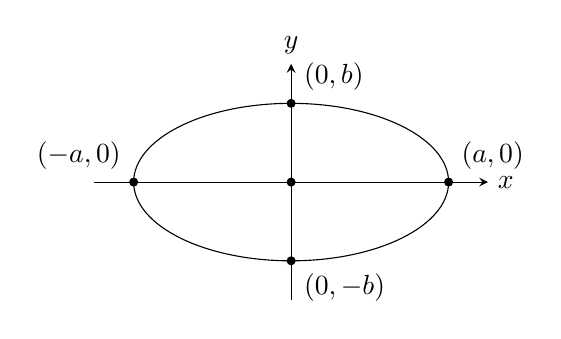
\begin{tikzpicture}
            % Set the values of a and b
            \def\a{2}
            \def\b{1}

            % Draw x and y axes
            \draw[-stealth] (-\a-0.5,0) -- (\a+0.5,0) node[right] {$x$};
            \draw[-stealth] (0,-\b-0.5) -- (0,\b+0.5) node[above] {$y$};
            
            % Plot the ellipse
            \draw (0,0) ellipse ({\a} and {\b});
            
            % Add labels or additional features if needed
            \node[draw,fill,circle,inner sep=1pt] at (0,0) {};
            \node[draw,fill,circle,inner sep=1pt,label={above right:$(a,0)$}] at (\a,0) {};
            \node[draw,fill,circle,inner sep=1pt,label={above left:$(-a,0)$}] at (-\a,0) {};
            \node[draw,fill,circle,inner sep=1pt,label={above right:$(0,b)$}] at (0,\b) {};
            \node[draw,fill,circle,inner sep=1pt,label={below right:$(0,-b)$}] at (0,-\b) {};

            
            \end{tikzpicture}
            \caption{Elipse.}
            \label{fig:Elipse}
    \end{figure}
    
    \item $\displaystyle \frac{x^2}{a^2} + \frac{y^2}{b^2} = 0$.

    Tenemos que es un único punto, el origen: $H=\{(0,0)\}$.
    
    \item $\displaystyle \frac{x^2}{a^2} - \frac{y^2}{b^2} = -1$.

    Se trata de una hipérbola. Calculemos sus puntos de corte:
    \begin{equation*}
        \left\{\begin{array}{l}
            x=0 \Longrightarrow y=\pm b  \\
            y=0 \Longrightarrow \nexists
        \end{array}\right.
    \end{equation*}

    Por tanto, tan solo corta al eje $Y$. Calculemos sus asíntotas oblicuas\footnote{Aunque este concepto no se haya introducido en la carrera de Matemáticas, se da por conocido de Bachillerato solo con el objeto de hacer ver que se trata de una hipérbola}. Tenemos que $y=f(x)=\pm b\sqrt{1+\frac{x^2}{a^2}}$. Si la asíntota oblicua es $y=mx+n$, calculamos $m,n$:
    \begin{equation*}
        m = \lim_{x\to \infty} \frac{f(x)}{x} = \lim_{x\to \infty} \frac{\pm b\sqrt{1+\frac{x^2}{a^2}}}{x}
        = \lim_{x\to \infty} \pm b\sqrt{\frac{1}{x^2}+\frac{1}{a^2}} = \pm \frac{b}{a}
    \end{equation*}
    \begin{multline*}
        n = \lim_{x\to \infty} f(x) -mx
        = \lim_{x\to \infty} \pm b\sqrt{1+\frac{x^2}{a^2}} \mp \frac{bx}{a} 
        = \lim_{x\to \infty} \pm b\left[\sqrt{1+\frac{x^2}{a^2}} - \frac{x}{a}\right]
        =\\= \lim_{x\to \infty} \dfrac{\pm b\left[{1+\cancel{\frac{x^2}{a^2}}} -\cancel{ \frac{x^2}{a^2}}\right]}{\sqrt{1+\frac{x^2}{a^2}} + \frac{x}{a}} = 0
    \end{multline*}

    Por tanto, tenemos que tiene dos asíntotas oblicuas, $y=\pm \frac{b}{a}x$. Está representada en la Figura \ref{fig:HiperbolaCortaY}.
    \begin{figure}
        \centering
        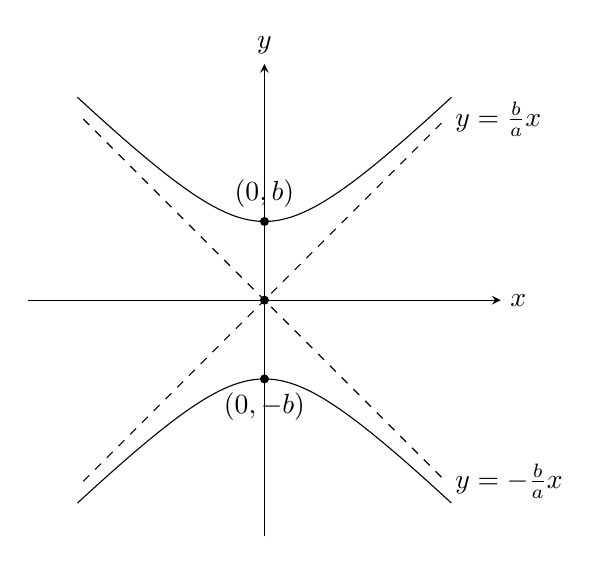
\begin{tikzpicture}
            % Set the values of a and b for the hyperbola
            \def\a{1}
            \def\b{1}
            
            % Plot the hyperbola
            \draw plot[domain=-1.6:1.6, samples=100] ({\a*sinh(\x)}, {\b*cosh(\x)});
            \draw plot[domain=-1.6:1.6, samples=100] ({\a*sinh(\x)}, {-\b*cosh(\x)});
            
            
            % Draw x and y axes
            \draw[-stealth] (-\a-2,0) -- (\a+2,0) node[right] {$x$};
            \draw[-stealth] (0,-\b-2) -- (0,\b+2) node[above] {$y$};
            
            % Draw asymptotes
            \draw[dashed] (-2.3,-2.3) -- (2.3,2.3) node[right] {$y = \frac{b}{a}x$};
            \draw[dashed] (-2.3, 2.3) -- (2.3, -2.3) node[right] {$y = -\frac{b}{a}x$};
            
            % Label the center and mark it with a dot
            \node[draw, fill, circle, inner sep=1pt] at (0,0) {};

            \node[draw,fill,circle,inner sep=1pt,label={above:$(0,b)$}] at (0,\b) {};
            \node[draw,fill,circle,inner sep=1pt,label={below:$(0,-b)$}] at (0,-\b) {};
        \end{tikzpicture}
        \caption{Hipérbola que corta al eje $Y$.}
        \label{fig:HiperbolaCortaY}
    \end{figure}
    
    \item $\displaystyle \frac{x^2}{a^2} - \frac{y^2}{b^2} = 1$.

    Se trata también de una hipérbola. Calculemos sus puntos de corte:
    \begin{equation*}
        \left\{\begin{array}{l}
            x=0 \Longrightarrow \nexists  \\
            y=0 \Longrightarrow x=\pm a
        \end{array}\right.
    \end{equation*}

    Por tanto, tan solo corta al eje $X$. Además, tiene las dos mismas dos asíntotas oblicuas, $y=\pm \frac{b}{a}x$. Está representada en la Figura \ref{fig:Hiperbola_CortaX}.
    \begin{figure}
        \centering
        \begin{tikzpicture}
            % Set the values of a and b for the hyperbola
            \def\a{1}
            \def\b{1}
            
            % Plot the hyperbola
            \draw plot[domain={-sqrt(\a^2 + 1)}:{sqrt(\a^2 + 1)}, samples=100] ({\a*cosh(\x)}, {\b*sinh(\x)});
            \draw plot[domain={-sqrt(\a^2 + 1)}:{sqrt(\a^2 + 1)}, samples=100] ({-\a*cosh(\x)}, {\b*sinh(\x)});
           
            
            % Draw x and y axes
            \draw[-stealth] (-\a-2,0) -- (\a+2,0) node[right] {$x$};
            \draw[-stealth] (0,-\b-2) -- (0,\b+2) node[above] {$y$};
            
            % Draw asymptotes
            \draw[dashed] (-2.3,-2.3) -- (2.3,2.3) node[right] {$y = \frac{b}{a}x$};
            \draw[dashed] (-2.3, 2.3) -- (2.3, -2.3) node[right] {$y = -\frac{b}{a}x$};
            
            % Label the center and mark it with a dot
            \node[draw, fill, circle, inner sep=1pt] at (0,0) {};
            \node[draw,fill,circle,inner sep=1pt,label={above right:$(a,0)$}] at (\a,0) {};
            \node[draw,fill,circle,inner sep=1pt,label={above left:$(-a,0)$}] at (-\a, 0) {};
        \end{tikzpicture}
        \caption{Hipérbola que corta al eje $X$.}
        \label{fig:Hiperbola_CortaX}
    \end{figure}

    
    \item $\displaystyle \frac{x^2}{a^2} - \frac{y^2}{b^2} = 0$.

    Tenemos que:
    \begin{equation*}
        0 = \frac{x^2}{a^2} - \frac{y^2}{b^2} = \left(\frac{x}{a}-\frac{y}{b}\right)\left(\frac{x}{a}+\frac{y}{b}\right)
    \end{equation*}

    Por tanto, se trata de un par de rectas secantes; representadas en la Figura \ref{fig:RectaDobleSec}.
    \begin{figure}
        \centering
        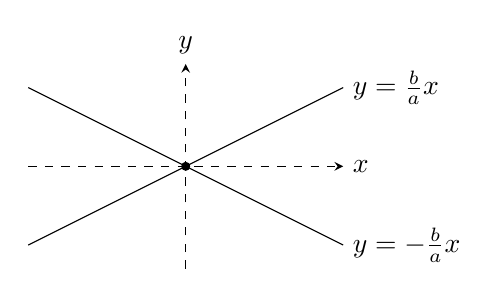
\begin{tikzpicture}

            % Draw x and y axes
            \draw[-stealth, dashed] (-2,0) -- (2,0) node[right] {$x$};
            \draw[-stealth, dashed] (0,-1.3) -- (0,1.3) node[above] {$y$};
            
            % Draw asymptotes
            \draw (-2,-1) -- (2,1) node[right] {$y = \frac{b}{a}x$};
            \draw (-2, 1) -- (2,-1) node[right] {$y = -\frac{b}{a}x$};
            
            % Label the center and mark it with a dot
            \node[draw, fill, circle, inner sep=1pt] at (0,0) {};
        \end{tikzpicture}
        \caption{Par de rectas secantes.}
        \label{fig:RectaDobleSec}
    \end{figure}
    
    \item $\displaystyle \frac{x^2}{a^2} = -1$.

    Tenemos que no es posible, por lo que $H=\emptyset$.
    \item $\displaystyle \frac{x^2}{a^2} = 1$

    Tenemos que:
    \begin{equation*}
        x^2 = a^2 \Longrightarrow x=\pm a
    \end{equation*}

    Por tanto, se trata de un par de rectas paralelas; representadas en la Figura \ref{fig:RectaDoblePar}.
    \begin{figure}
        \centering
        \begin{tikzpicture}
            \def\a{1}

            % Draw x and y axes
            \draw[-stealth] (-2,0) -- (2,0) node[right] {$x$};
            \draw[-stealth] (0,-1.3) -- (0,1.3) node[above] {$y$};
            
            \draw (-\a,-1) -- (-\a,1) node[above left] {$x=-a$};
            \draw (\a, -1) -- (\a,1) node[above right] {$x=a$};
        \end{tikzpicture}
        \caption{Par de rectas paralelas.}
        \label{fig:RectaDoblePar}
    \end{figure}
    
    \item $\displaystyle \frac{x^2}{a^2} = 0$.

    Tenemos que:
    \begin{equation*}
        x^2 = 0 \Longrightarrow x=0
    \end{equation*}

    Por tanto, se trata de una recta (doble); representada en la Figura \ref{fig:Recta}.
    \begin{figure}
        \centering
        \begin{tikzpicture}
            \def\a{0}

            % Draw x and y axes
            \draw[-stealth, dashed] (-2,0) -- (2,0);
            
            \draw[thick] (-\a,-1) -- (-\a,1) node[above] {$x=0$};
            \node[draw, fill, circle, inner sep=1pt] at (0,0) {};
        \end{tikzpicture}
        \caption{Recta (doble).}
        \label{fig:Recta}
    \end{figure}
    
    \item $\displaystyle \frac{x^2}{a^2} = 2y$.

    Tenemos que:
    \begin{equation*}
        y = \frac{x^2}{2a^2}
    \end{equation*}

    Por tanto, se trata de una parábola; representada en la Figura \ref{fig:Parabola}.
    \begin{figure}
        \centering
        \begin{tikzpicture}
            \def\a{1}

            % Draw x and y axes
            \draw[-latex] (-2.5,0) -- (2.5,0) node[right] {$x$};
            \draw[-latex] (0,-1) -- (0,3) node[above] {$y$};
            
            \draw plot[domain=-1.6:1.6, samples=100] (\x, {\a*\x*\x});
            \node[draw, fill, circle, inner sep=1pt] at (0,0) {};

        \end{tikzpicture}
        \caption{Parábola.}
        \label{fig:Parabola}
    \end{figure}
    
\end{enumerate}



\subsection{Clasificación de las cuádricas}

En esta sección, vamos a clasificar las hipercuádricas en el espacio euclídeo, también llamadas \textbf{cuádricas}\footnote{Estas posiblemente serán menos conocidas para el lector, pero son las equivalentes en el espacio.}.

Todas las cuádricas se pueden visulizar gráficamente en el siguiente applet de GeoGebra: \href{https://www.geogebra.org/m/bvgwetxk}{https://www.geogebra.org/m/bvgwetxk}.

Usando el Teorema \ref{teo:Clasif_Hiper}, podemos hacer la distinción de los posibles casos. Notemos que, como $R_i>0$ para todo $i$, y $f:\bb{R}^+\to \bb{R}^+$ dada por $f(x)=\frac{1}{x^2}$ es biyectiva, notemos que es indiferente poner $R_i$ que $\frac{1}{(R'_i)^2}$. Por tanto, los distintos casos son:
\begin{enumerate}
    \item $\dfrac{x^2}{a^2} + \dfrac{y^2}{b^2} + \dfrac{z^2}{c^2} = 0$.

    Se trata de un punto, el origen. $H=\{(0,0,0)\}$.
    
    \item $\dfrac{x^2}{a^2} + \dfrac{y^2}{b^2} + \dfrac{z^2}{c^2} = 1$.

    Se trata de un \ul{elipsoide de semiejes $a,b$ y $c$}.

    Vemos fácilmente que los cortes con cada plano son elipses.
    
    \item $\dfrac{x^2}{a^2} + \dfrac{y^2}{b^2} + \dfrac{z^2}{c^2} = -1$.

    No es posible, por lo que $H=\emptyset$.
    
    \item $\dfrac{x^2}{a^2} + \dfrac{y^2}{b^2} - \dfrac{z^2}{c^2} = 0$.

    Se trata de un \ul{cono elíptico}. Tenemos que:
    \begin{equation*}
        \dfrac{x^2}{a^2} + \dfrac{y^2}{b^2} = \dfrac{z^2}{c^2}
    \end{equation*}

    Por tanto, para cada valor de $z$, tenemos una elipse que crece de tamaño conforme lo hace $|z|$. Además, para $z=0$ tenemos un único punto, el origen.

    Veamos ahora los cortes con los planos $x=0$ e $y=0$:
    \begin{equation*}
        x = 0 \Longrightarrow \dfrac{y^2}{b^2} = \dfrac{z^2}{c^2} \Longrightarrow \left\{\begin{array}{c}
            y = \pm \frac{b}{c}z\\
            x=0
        \end{array}\right.
    \end{equation*}
    \begin{equation*}
        y = 0 \Longrightarrow \dfrac{x^2}{a^2} = \dfrac{z^2}{c^2} \Longrightarrow \left\{\begin{array}{c}
            x = \pm \frac{a}{c}z\\
            y=0
        \end{array}\right.
    \end{equation*}
    Por tanto, tenemos que son dos rectas en cada caso.
    
    \item $\dfrac{x^2}{a^2} + \dfrac{y^2}{b^2} - \dfrac{z^2}{c^2} = 1$.

    Se trata de un \ul{hiperboloide reglado o de una hoja}. Tenemos que:
    \begin{equation*}
        \dfrac{x^2}{a^2} + \dfrac{y^2}{b^2} = 1 + \dfrac{z^2}{c^2}
    \end{equation*}

    Por tanto, para cada valor de $z$, tenemos una elipse que crece de tamaño conforme lo hace $|z|$. Además, para $z=0$ también tenemos una elipse.

    Veamos ahora los cortes con los planos $x=0$ e $y=0$:
    \begin{gather*}
        x = 0 \Longrightarrow \dfrac{y^2}{b^2} - \dfrac{z^2}{c^2} = 1 \\
        y = 0 \Longrightarrow \dfrac{x^2}{a^2} - \dfrac{z^2}{c^2} = 1
    \end{gather*}
    Por tanto, tenemos que en cada caso es una hipérbola que no corta al eje $Z$.

    Veamos ahora por qué se llama ``reglado''. Tenemos que:
    \begin{equation*}
        \dfrac{x^2}{a^2} - \dfrac{z^2}{c^2} = 1 - \dfrac{y^2}{b^2} \Longrightarrow
        \left(\frac{x}{a}+\frac{z}{c}\right)\left(\frac{x}{a}-\frac{z}{c}\right)=
        \left(1+\frac{y}{b}\right)\left(1-\frac{y}{b}\right)
        \Longrightarrow
        \frac{\left(\frac{x}{a}-\frac{z}{c}\right)}{\left(1-\frac{y}{b}\right)} = \frac{\left(1+\frac{y}{b}\right)}{\left(\frac{x}{a}+\frac{z}{c}\right)}:=\mu
    \end{equation*}
    Por tanto, tenemos la siguiente familia de rectas:
    \begin{equation*}
        r_\lm \equiv \left\{
        \begin{array}{l}
            \left(\frac{x}{a}-\frac{z}{c}\right) = \mu\left(1-\frac{y}{b}\right)\\
            \left(1+\frac{y}{b}\right) = \mu\left(\frac{x}{a}+\frac{z}{c}\right)
        \end{array}
        \right.
    \end{equation*}
    Por ello, se llama hiperboloide reglado, ya que está formado por una familia de rectas.

    
    \item $\dfrac{x^2}{a^2} + \dfrac{y^2}{b^2} - \dfrac{z^2}{c^2} = -1$.

    Se trata de un \ul{hiperboloide elíptico o de dos hojas}. Tenemos que:
    \begin{equation*}
        \dfrac{x^2}{a^2} + \dfrac{y^2}{b^2} = -1 + \dfrac{z^2}{c^2}
    \end{equation*}

    Por tanto, para cada valor de $z$ tal que $|z|>c$, tenemos una elipse que crece de tamaño conforme lo hace $|z|$. Además, para $z=\pm c$, tenemos un único punto. Para $z\in ]-c,c[$, tenemos que no existe ningún punto de la cuádrica.

    Veamos ahora los cortes con los planos $x=0$ e $y=0$:
    \begin{gather*}
        x = 0 \Longrightarrow \dfrac{y^2}{b^2} - \dfrac{z^2}{c^2} = -1 \\
        y = 0 \Longrightarrow \dfrac{x^2}{a^2} - \dfrac{z^2}{c^2} = -1
    \end{gather*}
    Por tanto, tenemos que en cada caso es una hipérbola que corta al eje $Z$ y no corta a los otros ejes.

    
    \item $\dfrac{x^2}{a^2} + \dfrac{y^2}{b^2} = 0$.

    Tenemos que $H\equiv x=y=0$, por lo que se trata de una recta.
    
    \item $\dfrac{x^2}{a^2} + \dfrac{y^2}{b^2} = 1$.

    Para cada valor de $z$ tenemos la misma elipse, por lo que se trata de un \ul{cilindro elíptico}.
    
    \item $\dfrac{x^2}{a^2} + \dfrac{y^2}{b^2} = -1$.

    No es posible\footnote{Esta cuádrica también se denomina cilindro imaginario}, por lo que $H=\emptyset$.
    
    \item $\dfrac{x^2}{a^2} - \dfrac{y^2}{b^2} = 0$.

    Tenemos que:
    \begin{equation*}
        \left(\dfrac{x}{a} - \dfrac{y}{b}\right)\left(\dfrac{x}{a} + \dfrac{y}{b}\right) = 0 \Longrightarrow x = \pm \frac{a}{b}y
    \end{equation*}
    Por tanto, tenemos que son dos planos. Además, su intersección es la recta $x=y=0$; es decir, el eje $Z$.

    Por tanto, son \ul{dos planos secantes}.

    
    \item $\dfrac{x^2}{a^2} - \dfrac{y^2}{b^2} = 1$.

    Por tanto, para cada valor de $z$, tenemos la misma hipérbola que no corta al eje $Y$.

    Se denomina \ul{cilindro hiperbólico}.
    
    \item $\dfrac{x^2}{a^2} - \dfrac{y^2}{b^2} = -1$.

    Por tanto, para cada valor de $z$, tenemos la misma hipérbola que no corta al eje $X$.

    En este caso también se denomina \ul{cilindro hiperbólico}.
    
    \item $\dfrac{x^2}{a^2} = 0$.

    En este caso tengo $x=0$; por lo que es un \ul{plano (doble)}.
    
    \item $\dfrac{x^2}{a^2} = 1$.

    En este caso tengo $x=\pm a$; por lo que es un \ul{par de planos paralelos}.
    
    \item $\dfrac{x^2}{a^2} = -1$.

    No es posible, por lo que $H=\emptyset$.
    
    \item $\dfrac{x^2}{a^2} + \dfrac{y^2}{b^2} = 2z$.

    Se trata de un \ul{paraboloide elíptico}. 
    
    Para cada valor de $z>0$, tenemos una elipse que crece de tamaño conforme lo hace $z$. Para $z=0$ tenemos un único punto, el origen; y para $z<0$ tenemos que no es posible.

    Veamos ahora los cortes con los planos $x=0$ e $y=0$:
    \begin{equation*}
        x = 0 \Longrightarrow \dfrac{y^2}{b^2} = 2z \Longrightarrow z=\dfrac{y^2}{2b^2}
    \end{equation*}
    \begin{equation*}
        y = 0 \Longrightarrow \dfrac{x^2}{a^2} = 2z \Longrightarrow z=\dfrac{x^2}{2a^2}
    \end{equation*}
    Por tanto, tenemos que son dos parábolas en cada caso.
    
    
    \item $\dfrac{x^2}{a^2} - \dfrac{y^2}{b^2} = 2z$.

    Se trata de un \ul{paraboloide hiperbólico}. 
    
    Para cada valor de $z>0$, tenemos una hipérbola que corta al plano $y=0$ que con valores de los semiejes distintos. 
    
    Para $z=0$, tenemos dos rectas secantes, $r\equiv \left\{\begin{array}{l}
        z=0  \\
        y = \pm \frac{b}{a}x 
    \end{array}\right.$ 
    
    Para cada valor de $z<0$, tenemos una hipérbola que corta al plano $x=0$ que con valores de los semiejes distintos. 

    Veamos ahora los cortes con los planos $x=0$ e $y=0$:
    \begin{equation*}
        x = 0 \Longrightarrow \dfrac{y^2}{b^2} = -2z \Longrightarrow z=-\dfrac{y^2}{2b^2}
    \end{equation*}
    \begin{equation*}
        y = 0 \Longrightarrow \dfrac{x^2}{a^2} = 2z \Longrightarrow z=\dfrac{x^2}{2a^2}
    \end{equation*}
    Por tanto, tenemos que son dos parábolas en cada caso, una cóncava hacia arriba y otra cóncava hacia abajo.
    
    \item $\dfrac{x^2}{a^2} = 2z$.

    Para cualquier $y$, se tiene que:
    \begin{equation*}
        z = \dfrac{x^2}{2a^2}
    \end{equation*}

    Es decir, tenemos que es siempre la misma parábola. Se denomina \ul{cilindro parabólico}.
\end{enumerate}


















\begin{comment}
Recordemos el Teorema de Sylvester, que sirve para diagonzalizar matrices simétricas:
\begin{teo}[Sylvester]
    Sea $M\in \cc{S}_n(\bb{R})$. Entonces, existe una matriz regular $P$ de orden $n$ tal que:
    \begin{equation*}
        P^tMP = \left(\begin{array}{ccc}
            -I_a &  \\
             & I_b \\
             && 0_c
        \end{array}\right)
    \end{equation*}
    donde $a$ es el índice de $M$, $c$ su nulidad; y $a+b+c=n$.
\end{teo}

Además, contamos con esta conocida regla:
\begin{lema}[Descartes]
    El número de raíces positivas de un polinomio con coeficientes reales ordenados es, como máximo, el número de cambios de signo entre sus coeficientes.
\end{lema}

\begin{teo}
    Sea $f:\bb{R}^n \to \bb{R}^n$ una biyección afín y $C$ una hipercuádrica. Entonces, $f(C)$ es otra hipercuádrica.
\end{teo}

\begin{definicion}
    Dos hipercuádricas $C_1$ y $C_2$ de $\bb{R}^n$ se dicen equivalentes si existe una biyección afín $f : \bb{R}^n \to \bb{R}^n$ tal que $f(C_1) = C_2$.
\end{definicion}
\end{comment}







\section{Relación de Ejercicios}

Para ver ejercicios relacionados con este tema, consultar la sección \ref{Rel:Tema3}.